


\section{MLL}



\begin{figure}
\[
\begin{array}{llll}
	\MLLrule b
 &	\MLLrule 1
 &	\MLLrule p
 &	\MLLrule t
\end{array}
\]
\caption{Inference rules for unit-only \MLL}
\label{fig:MLL}
\end{figure}



\begin{figure}
\[
	\vc{\MLLperm{bb1}} \perm \vc{\MLLperm{bb2}}
\qquad
	\vc{\MLLperm{bp1}} \perm \vc{\MLLperm{bp2}}
\]
\[
	\vc{\MLLperm{bt1}} \perm \vc{\MLLperm{bt2}} \perm \vc{\MLLperm{bt3}}
\]
\[
	\vc{\MLLperm{pp1}} \perm \vc{\MLLperm{pp2}}
\]
\[
	\vc{\MLLperm{pt1}} \perm \vc{\MLLperm{pt2}}
\]
\[
	\vc{\MLLperm{tt1}} \perm \vc{\MLLperm{tt2}}
\]
\caption{Permutations}
\label{fig:permutations}
\end{figure}



The formulae of unit-only multiplicative linear logic are given by the following grammar.
%
\[
	A,B,C \coloneq \bot \mid 1 \mid A\parr B \mid A\tn B
\]
%
The connectives $\tn$ and $\parr$ will be considered up to associativity, and \emph{duality} $\dual A$ is via DeMorgan.
%
A \emph{sequent} $\Gamma,\Delta$ will be a multiset of formulae.
%
Within a sequent, connectives and units will be \emph{named} with distinct elements from an arbitrary set of names $N$, e.g.\
$\named a1\named b\parr\named c1,\named d\bot\named e\tn\named f\bot$.
%
This allows to 1) avoid using the notion of \emph{occurrence}, and instead refer to subformulae by the name of their root connective, as e.g.\ $\named bA$, 2) distinguish the two proofs of the above sequent while using standard multiset sequents, and 3) easily extract proof nets, as graphs using the names of connectives as vertices.
%
Names will mostly be left implicit.



Proofs are constructed from the inference rules in Figure~\ref{fig:MLL}.
%
The names of connectives are preserved through inferences.
%
Only cut-free proofs are considered, and no cut-rule is added.
%
\emph{Permutations} of inference rules are displayed in Figure~\ref{fig:permutations}; the symmetric variants of the last two permutations, \emph{par-tensor} and \emph{tensor-tensor}, have been omitted.



\begin{definition}
\label{def:equivalence}
%
\emph{Equivalence} of proofs in (cut-free, unit-only) multiplicative linear logic $(\perm)$ is the congruence generated by the permutations given in Figure~\ref{fig:permutations}.
%
\emph{\MLL\ proof equivalence} is the problem of deciding whether two given proofs are equivalent.
%
\end{definition}



The motivation to consider proofs up to equivalence is three-fold.
%
Firstly, there is the strong intuition that the order of permutable inferences does not contribute to the essential content of the proof.
%
Secondly, a technical motivation is that cut-elimination in \MLL\ incorporates permutation steps, and composition via cut-elimination is only associative up to permutations.
%
Thirdly, equivalent proofs are identified in natural models of multiplicative linear logic such as coherence spaces, and in the categorical semantics of \MLL, $\star$-autonomous categories.



In one of several possible definitions, a \emph{$\star$-autonomous category} \citep{Barr-1979} is a symmetric monoidal category $(\mathcal C,\tn,1)$ with:
%
\begin{itemize}
	
	\item
	a \emph{duality}, a contravariant functor $\dual-$ such that $A\cong\dual*A$, and

	\item
	\emph{closure}, an adjunction $-\tn B \dashv \dual{(B\tn\dual-)}$ for any object $B$,

\end{itemize}
%
satisfying natural coherence conditions.
%
%The category $\textsc{mll}(\emptyset)$ of unit-only \MLL-formulae and equivalence classes of proofs is a $\star$-autonomous category.
%
The category with as objects unit-only \MLL-formulae and as morphisms $A\to B$ the equivalence classes of proofs of $\dual A\parr B$, denoted $\textsc{mll}(\emptyset)$, is a $\star$-autonomous category.
%
The present formulation of formulae induces two forms of \emph{strictness}, instances where isomorphisms of the definition are identities: DeMorgan duality means $A=\dual*A$, while
%, one-sided sequents mean the closure adjunction is an equivalence of categories, 
associativity is an identity by decree.
%
Modulo strictness, $\textsc{mll}(\emptyset)$ is the \emph{free} $\star$-autonomous category over the empty category $\emptyset$.
%
This means that \emph{any} $\star$-autonomous category is a model of the logic, and that \MLL\ proof equivalence is the \emph{word problem} for $\star$-autonomous categories, the problem of deciding when two representations of morphisms denote the same morphism.




%The \emph{free $\star$-autonomous completion} $\star$-\textsc a$(\mathcal C)$ of a category $\mathcal C$ is characterised by a functor $i\colon\mathcal C\to\star$-\textsc a$(\mathcal C)$ such that any functor $\mathcal C\to \mathcal D$ into a $\star$-autonomous cateogry $\D$ factors uniquely (up to canonical isomorphism) as the composition of $i$ with a functor $\star$-\textsc a$(\mathcal C)\to\D$ preserving $\star$-autonomous structure.
%%
%\[
%\begin{tikzpicture}[auto]
%	\node (C) at (0,0) {$\mathcal C$};
%	\node (*AC) at (2,0) {$\star$-\textsc a$(\mathcal C)$};
%	\node (D) at (1,1) {$\mathcal D$};
%	\draw [->] (C) -- node {$i$} (*AC);
%	\draw [->] (C) -- (D);
%	\draw [->,dashed] (*AC) -- node {$!$} (D);
%\end{tikzpicture}
%\]
%%



\subsection{Proof nets}

A partial solution to the \MLL\ proof equivalence problem is provided by proof nets.


\begin{definition}
\label{def:proof nets}
%
For a sequent $\Gamma$,
\begin{itemize}

	\item
	a \emph{linking} $\links$ is a function from the names of $\bot$-subformulae to the names of $1$-subformulae,

	\item
	a \emph{switching graph} for $\links$ is an undirected graph over the names of $\Gamma$, with for every subformula $\named aA\named c\tn\named bB$ the edges $a-c$ and $b-c$, for every subformula $\named aA\named c\parr\named bB$ either the edge $a-c$ or the edge $b-c$, and for every subformula $\named a\bot$ the edge $a-\links(a)$,

 	\item
	a \emph{proof net} $\links$ or $(\Gamma,\links)$ is a linking $\links$ such that every switching graph is acyclic and connected.

\end{itemize}
\end{definition}


\noindent
An edge $a-\links(a)$ in a proof net or switching graph is a \emph{link} or \emph{jump}.



\begin{definition}
\label{def:proof net equivalence}
%
A \emph{permutation} between proof nets is the redirection of exactly one link.
%
\emph{Equivalence} $(\perm)$ of proof nets over a sequent $\Gamma$ is the congruence generated by permutations.
%
\end{definition}


\noindent
There is no canonical interpretation of a proof as a proof net, since the introduction rule for $\bot$ in proofs joins a $\bot$-formula to a sequent, rather than a formula.



\begin{definition}
\label{def:proofs to nets}
%
The relation $(\toNet)$ interprets a proof $\Pi$ for a sequent $\Gamma$ by a linking $\links$ as follows:
% 
$\Pi\toNet\links$ if for each $\named a\bot$ in $\Gamma$, if $\Delta$ is the context of the inference introducing $\named a\bot$, as illustrated below, then $\links(a)$ is the name of some $1$ in $\Delta$.
\[
	\infer[\MLLlabel b]{\Delta,\named a\bot}{\Delta}
\]
%
\end{definition}



\begin{proposition}[\citeauthor{DR89}, \citeyear{DR89}]
\label{prop:correctness and sequentialisation}
%
For a proof $\Pi$ with conclusion $\Gamma$, if $\Pi\toNet\links$ then $\links$ is a proof net for $\Gamma$.
%
For a net $\links$ for $\Gamma$, there is a proof $\Pi$ of $\Gamma$ such that $\Pi\toNet\links$ (\emph{sequentialisation}).
%
\end{proposition}


\noindent
Proof nets are canonical representations of proofs in the absence of units: they factor out the permutations among tensor- and par-inferences, which are the last three permutations in Figure~\ref{fig:permutations}.
%
Equivalence of proof nets is generated by the remaining equations, the permutations on $\bot$-introduction.



\begin{proposition}[\citeauthor{HughesMLLProofNets}, \citeyear{HughesMLLProofNets}]
\label{prop:proof nets work}
%
For proofs $\Pi$, $\Pi'$ and proof nets $\links$, $\links'$ such that $\Pi\toNet\links$ and $\Pi'\toNet\links'$, $\Pi\perm\Pi'$ if and only if $\links\perm\links'$.
%
\end{proposition}


\noindent
\MLL\ proof equivalence is the problem of deciding equivalence of proof nets.


\subsection{Notation}


We will use a concise diagrammatic notation for sequents and proof nets.
%
The units $1$ and $\bot$ are represented by a circle $\circ$ and a disc $\bullet$ respectively.
%
A tensor is represented by a line connecting both subformulae, and a par by juxtaposition: if $A$ and $B$ are represented by \raisebox{-0.3\height}{
\includegraphics[scale=0.75]{hex-A.pdf}}
and \raisebox{-0.3\height}{
\includegraphics[scale=0.75]{hex-B.pdf}},
%
then $A\parr B$ is \raisebox{-0.3\height}{
\includegraphics[scale=0.75]{hex-AparB.pdf}}
and $A\tn B$ is \raisebox{-0.3\height}{
\includegraphics[scale=0.75]{hex-AtnB.pdf}}.
%
A tensor of multiple elements is denoted by stringing them together in a line, so $A\tn B\tn C$ is
\raisebox{-0.3\height}{
\includegraphics[scale=0.75]{hex-AtnBtnC.pdf}}.
%
Boxes play the role of parentheses around par-formulae, so $(A\parr B)\tn C$ is drawn as \begin{center}{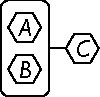
\includegraphics[scale=1]{hex-AparBtnC.pdf}}\end{center}

\noindent For example, this sequent
\[ \vdash \bot\tn\bot, \bot\tn\bot, \bot\tn\bot, \bot\tn\bot, 1, \{[(1\parr 1\parr 1)\tn(1\parr 1\parr 1)]\parr 1\parr (\bot\tn\bot\tn\bot)\parr 1\}\tn\bot \]
could be drawn like this:
\begin{center}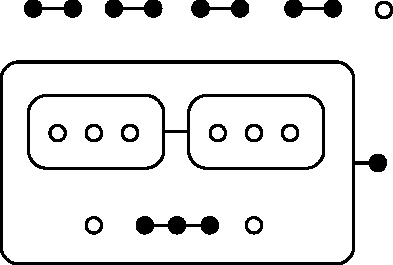
\includegraphics[scale=0.75]{example-sequent.pdf}\end{center}

\noindent We represent a proof net by drawing an arrow from each $\bullet$ to some $\circ$. For example, one proof net on the above sequent is
\begin{center}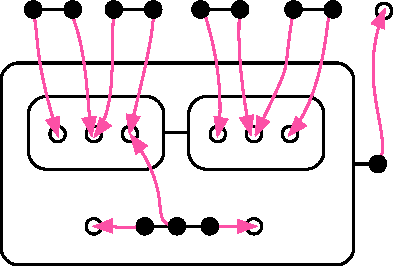
\includegraphics[scale=0.75]{example-sequent-proofnet.pdf}\end{center}







